\chapter{The \Vaango framework}

\section{Historical information}
\Vaango is a fork of the Uintah Computational Framework (\Uintah) created
in 2012 to allow for the development of tools to solve solid mechanics problems
in mechanical and civil engineering.
The orginal \Uintah code continues to be actively developed, but the focus
of that code is multiphysics problems, particularly computational fluid
dynamics (CFD) and chemical engineering.  Around once a year, the underlying 
parallel computing infrastructure of \Vaango is updated to keep up with 
developments in \Uintah.

The \Vaango framework, like \Uintah, consists of a
set of software components and libraries that facilitate the solution
of Partial Differential Equations (PDEs) on Structured AMR (SAMR)
grids using hundreds to thousands of processors.  However, unlike the
CFD problems that \Uintah was designed for, the use of the grid is
often only incidental to the solution of the governing PDEs of solid
mechanics.

\section{Overview}
One of the challenges in designing a parallel, component-based
multi-physics application is determining how to efficiently decompose
the problem domain. Components, by definition, make local
decisions. Yet parallel efficiency is only obtained through a globally
optimal domain decomposition and scheduling of computational
tasks. Typical techniques include allocating disjoint sets of
processing resources to each component, or defining a single domain
decomposition that is a compromise between the ideal load balance of
multiple components. However, neither of these techniques will achieve
maximum efficiency for complex multi-physics problems.

\Vaango uses a non-traditional approach to achieving parallelism,
employing an abstract taskgraph representation to describe computation
and communication. The taskgraph is an explicit representation of the
computation and communication that occur in the coarse of a single
iteration of the simulation (typically a timestep or nonlinear solver
iteration) see figure~\ref{fig:TaskGraph}. \Vaango components delegate
decisions about parallelism to a scheduler component, using variable
dependencies to describe communication patterns and characterizing
computational workloads to facilitate a global resource
optimization. The taskgraph representation has a number of advantages,
including efficient fine-grained coupling of multi-physics components,
flexible load balancing mechanisms and a separation of application
concerns from parallelism concerns. However, it creates a challenge
for scalability which we overcome by creating an implicit definition
of this graph and representing it in a distributed fashion.

\begin{figure}
  \centering
  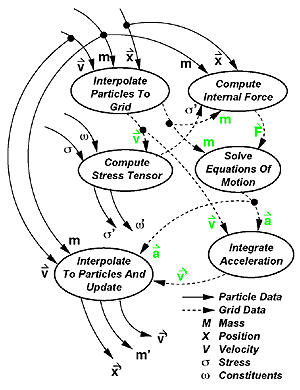
\includegraphics[width=0.5\textwidth]{Taskgraph-diagram.png}
  \caption{Example Task Graph}
  \label{fig:TaskGraph}
\end{figure}

The primary advantage of a component-based approach is that it
facilitates the separate development of simulation algorithms, models,
and infrastructure. Components of the simulation can evolve
independently. The component-based architecture allows pieces of the
system to be implemented in a rudimentary form at first and then
evolve as the technologies mature. Most importantly, \Vaango allows the
aspects of parallelism (schedulers, load-balancers, parallel
input/output, and so forth) to evolve independently of the simulation
components. Furthermore, components enable replacement of computation
pieces without complex decision logic in the code itself.

\section{An example}
The sequence of steps performed in a simulation can be seen in the
abbreviated example below.  A complete version of this example can be 
found in the unit test for \Textsfc{TabularPlasticity}  located
at \Textsfc{src/CCA/Components/MPM/ConstitutiveModel/UnitTests/testTabularPlasticity.cc}.

\begin{lstlisting}[language=Cpp]
 try {
    // Read the input file
    ProblemSpecP ups = VaangoEnv::createInput();
    ups->getNode()->_private = (void *) ups_file.c_str();

    // Create the MPI/threading environment
    const ProcessorGroup* world = Uintah::Parallel::getRootProcessorGroup();

    // Create the simulation controller
    SimulationController* ctl = scinew AMRSimulationController(world, false, ups);
    
    // Create a regridder if needed
    RegridderCommon* reg = 0;

    // Create an implicit solver if needed
    SolverInterface* solve = SolverFactory::create(ups, world, "");

    // Create the component for the simulation (MPM/MPMICE/Peridynamics)
    UintahParallelComponent* comp = ComponentFactory::create(ups, world, false, "");

    // Create the simulation base object
    SimulationInterface* sim = dynamic_cast<SimulationInterface*>(comp);
    ctl->attachPort("sim", sim);
    comp->attachPort("solver", solve);
    comp->attachPort("regridder", reg);

    // Create a load balancer
    LoadBalancerCommon* lbc = LoadBalancerFactory::create(ups, world);
    lbc->attachPort("sim", sim);

    // Create a data archiver
    DataArchiver* dataarchiver = scinew DataArchiver(world, -1);
    Output* output = dataarchiver;
    ctl->attachPort("output", dataarchiver);
    dataarchiver->attachPort("load balancer", lbc);
    comp->attachPort("output", dataarchiver);
    dataarchiver->attachPort("sim", sim);

    // Create a task scheduler
    SchedulerCommon* sched = SchedulerFactory::create(ups, world, output);
    sched->attachPort("load balancer", lbc);
    ctl->attachPort("scheduler", sched);
    lbc->attachPort("scheduler", sched);
    comp->attachPort("scheduler", sched);
    sched->setStartAddr( start_addr );
    sched->addReference();

    // Run the simulation
    ctl->run();

    // Clean up after the simulation is complete
    delete ctl;
    sched->removeReference();
    delete sched;
    delete lbc;
    delete sim;
    delete solve;
    delete output; 

  } catch (ProblemSetupException& e) {
    std::cout << e.message() << std::endl;
    thrownException = true;
  } catch (Exception& e) {
    std::cout << e.message() << std::endl;
    thrownException = true;
  } catch (...) {
    std::cout << "**ERROR** Unknown exception" << std::endl;
    thrownException = true;
  }
\end{lstlisting}
